% Options for packages loaded elsewhere
\PassOptionsToPackage{unicode}{hyperref}
\PassOptionsToPackage{hyphens}{url}
%
\documentclass[conference]{IEEEtran}
\usepackage{amsmath,amssymb}
\usepackage{iftex}
\ifPDFTeX
  \usepackage[T1]{fontenc}
  \usepackage[utf8]{inputenc}
  \usepackage{textcomp} % provide euro and other symbols
\else % if luatex or xetex
  \usepackage{unicode-math} % this also loads fontspec
  \defaultfontfeatures{Scale=MatchLowercase}
  \defaultfontfeatures[\rmfamily]{Ligatures=TeX,Scale=1}
\fi
\usepackage{lmodern}
\ifPDFTeX\else
  % xetex/luatex font selection
\fi
% Use upquote if available, for straight quotes in verbatim environments
\IfFileExists{upquote.sty}{\usepackage{upquote}}{}
\IfFileExists{microtype.sty}{% use microtype if available
  \usepackage[]{microtype}
  \UseMicrotypeSet[protrusion]{basicmath} % disable protrusion for tt fonts
}{}
\makeatletter
\@ifundefined{KOMAClassName}{% if non-KOMA class
  \IfFileExists{parskip.sty}{%
    \usepackage{parskip}
  }{% else
    \setlength{\parindent}{0pt}
    \setlength{\parskip}{6pt plus 2pt minus 1pt}}
}{% if KOMA class
  \KOMAoptions{parskip=half}}
\makeatother
\usepackage{xcolor}
\usepackage{longtable,booktabs,array}
\usepackage{calc} % for calculating minipage widths
% Correct order of tables after \paragraph or \subparagraph
\usepackage{etoolbox}
\makeatletter
\patchcmd\longtable{\par}{\if@noskipsec\mbox{}\fi\par}{}{}
\makeatother
% Allow footnotes in longtable head/foot
\IfFileExists{footnotehyper.sty}{\usepackage{footnotehyper}}{\usepackage{footnote}}
\makesavenoteenv{longtable}
\usepackage{graphicx}
\makeatletter
\def\maxwidth{\ifdim\Gin@nat@width>\linewidth\linewidth\else\Gin@nat@width\fi}
\def\maxheight{\ifdim\Gin@nat@height>\textheight\textheight\else\Gin@nat@height\fi}
\makeatother
% Scale images if necessary, so that they will not overflow the page
% margins by default, and it is still possible to overwrite the defaults
% using explicit options in \includegraphics[width, height, ...]{}
\setkeys{Gin}{width=\maxwidth,height=\maxheight,keepaspectratio}
% Set default figure placement to htbp
\makeatletter
\def\fps@figure{htbp}
\makeatother
\setlength{\emergencystretch}{3em} % prevent overfull lines
\providecommand{\tightlist}{%
  \setlength{\itemsep}{0pt}\setlength{\parskip}{0pt}}
\setcounter{secnumdepth}{-\maxdimen} % remove section numbering
\ifLuaTeX
  \usepackage{selnolig}  % disable illegal ligatures
\fi
\usepackage{bookmark}
\IfFileExists{xurl.sty}{\usepackage{xurl}}{} % add URL line breaks if available
\urlstyle{same}
\hypersetup{
  hidelinks,
  pdfcreator={LaTeX via pandoc}}

\title{From Reactive to Proactive: An AI-Driven Early Warning System for Enhancing Supply Chain Resilience Through News-Operational Data Fusion}

\author{\IEEEauthorblockN{Duc-Duong Dao Minh\IEEEauthorrefmark{1}, Buu-Tanh Tran-Le, Huyen-Huynh Chau Nhu,\\Thuy-Nguyen Nhut, Linh-Le Quynh Khanh}
\IEEEauthorblockA{University of Economics and Law, Ho Chi Minh City, Vietnam\\
\IEEEauthorrefmark{1}Corresponding author. E-mail: ducdmk24406@st.uel.edu.vn}}
\date{}

\begin{document}

\maketitle

\begin{abstract}
Existing supply chain disruption forecasting approaches remain confined to a single data modality, leaving a critical blind-spot: no validated pipeline demonstrates whether fusing heterogeneous modalities yields measurable Incremental Predictive Validity over unimodal baselines. This study proposes a four-stage Cascading AI architecture that transforms raw logistics news into calibrated risk features via DistilBERT-based binary filtering and zero-shot multi-label classification, then fuses them with structured ERP data through a Geographic Weighting function before training gradient-boosted classifiers. Experiments on 8,728 logistics news articles (2022--2024) and five aerospace operational datasets yield three principal findings: (1) the Gatekeeper binary filter achieves ROC-AUC = 0.8927 and Recall = 0.9503; (2) the fused XGBoost model attains Precision = 0.1654 on minority-class stockout prediction --- a 28.7\% relative improvement over the ERP-only baseline, substantiating Incremental Predictive Validity; and (3) the system provides a Lead-Time Gain of 1.0 to 3.2 weeks across all component families prior to disruption onset. These results validate that integrating public-domain textual signals with operational telemetry produces an actionable early warning capability for upstream inventory risk.
\end{abstract}

\begin{IEEEkeywords}
Supply Chain Risk Management, Natural Language Processing, Heterogeneous Data Fusion, Early Warning System, Inventory Disruption Forecasting
\end{IEEEkeywords}

\subsection{1. Introduction}\label{introduction}

\subsubsection{1.1. Motivation and Operational
Context}\label{motivation-and-operational-context}

The grounding of the container vessel \emph{Ever Given} in the Suez
Canal (March 2021) --- incurring an estimated USD 9.6 billion in trade
losses over six days --- exposed a structural fragility that subsequent
crises have only reinforced. The 2021--2023 semiconductor shortage
cascade compelled aerospace and automotive manufacturers to curtail
production, while the Red Sea shipping diversions of 2024
re-demonstrated that single-point-of-failure vulnerabilities propagate
nonlinearly through multi-tier supply networks. Gartner (2023) reports
that 87\% of manufacturing enterprises experienced at least one material
supply disruption between 2020 and 2023.

The critical operational challenge is temporal: risk signals --- port
congestion reports, labor dispute announcements, geopolitical sanction
notices --- typically surface in the public information environment
\emph{before} their consequences materialize as inventory depletion or
assembly-line stoppages. The interval between the earliest detectable
exogenous signal and the onset of operational impact constitutes the
actionable early warning window. Converting this latent informational
lead into a reliable, quantified decision support instrument remains an
unsolved problem in Supply Chain Risk Management (SCRM).

\subsubsection{1.2. Research Problem}\label{research-problem}

The prevailing industrial practice for upstream risk monitoring relies
on reactive mechanisms: periodic procurement reports, manual scanning of
trade press, and threshold-based key performance indicators (KPIs)
derived from ERP systems. These methods detect disruptions only
\emph{post-facto} --- after inventory buffers are exhausted or delivery
commitments are missed --- and fundamentally cannot leverage the
high-volume, high-velocity textual data published daily across global
logistics news portals. The operational cost of this reactive posture is
asymmetric: the economic penalty for a missed disruption (false
negative) vastly exceeds the cost of investigating a spurious alert
(false positive), yet existing monitoring architectures are not
calibrated to reflect this cost asymmetry.

\subsubsection{1.3. Research Gap}\label{research-gap}

A systematic examination of the SCRM literature reveals a persistent
Modality Decoupling problem: studies either exploit unstructured textual
data without connecting to internal operational states, or analyze
structured ERP data while remaining blind to exogenous environmental
signals. Table 1 synthesizes this gap across four representative
state-of-the-art (SOTA) contributions. Critically, no prior work
simultaneously satisfies three conditions: (a) heterogeneous modality
fusion of NLP-derived and ERP-derived features within a unified
pipeline; (b) spatial risk sensitivity calibration to resolve the
granularity mismatch between macro-level news (country-level) and
micro-level ERP (supplier-level); and (c) rigorous demonstration of
Incremental Predictive Validity --- empirical evidence that the fused
model outperforms the unimodal baseline, not merely that it ingests more
data.

\textbf{Table 1.} Positioning matrix: contribution comparison with
representative SOTA studies.

\begin{longtable}[]{@{}
  >{\raggedright\arraybackslash}p{(\columnwidth - 10\tabcolsep) * \real{0.1071}}
  >{\centering\arraybackslash}p{(\columnwidth - 10\tabcolsep) * \real{0.1786}}
  >{\centering\arraybackslash}p{(\columnwidth - 10\tabcolsep) * \real{0.1786}}
  >{\centering\arraybackslash}p{(\columnwidth - 10\tabcolsep) * \real{0.1786}}
  >{\centering\arraybackslash}p{(\columnwidth - 10\tabcolsep) * \real{0.1786}}
  >{\centering\arraybackslash}p{(\columnwidth - 10\tabcolsep) * \real{0.1786}}@{}}
\toprule\noalign{}
\begin{minipage}[b]{\linewidth}\raggedright
Evaluation Criterion
\end{minipage} & \begin{minipage}[b]{\linewidth}\centering
Cano-Marin et al.~(2023)
\end{minipage} & \begin{minipage}[b]{\linewidth}\centering
Ivanov et al.~(2022)
\end{minipage} & \begin{minipage}[b]{\linewidth}\centering
J. Wang (2024)
\end{minipage} & \begin{minipage}[b]{\linewidth}\centering
Brintrup et al.~(2020)
\end{minipage} & \begin{minipage}[b]{\linewidth}\centering
\textbf{Present Study}
\end{minipage} \\
\midrule\noalign{}
\endhead
\bottomrule\noalign{}
\endlastfoot
NLP-derived risk signals & ✓ & ✗ & ✓ & ✗ & \textbf{✓} \\
Internal operational data integration & ✗ & ✓ & ✗ & ✓ & \textbf{✓} \\
Heterogeneous modality fusion & ✗ & ✗ & Partial & ✗ & \textbf{✓} \\
Spatial risk sensitivity mapping & ✗ & ✗ & ✗ & ✗ & \textbf{✓} \\
Demonstrated incremental predictive validity & ✗ & ✗ & Partial & ✗ &
\textbf{✓} \\
Walk-forward temporal validation & ✗ & ✗ & ✗ & ✓ & \textbf{✓} \\
\end{longtable}

\subsubsection{1.4. Objectives and
Contributions}\label{objectives-and-contributions}

This study advances three contributions that directly address the
methodological barriers identified above:

\textbf{(C1) Heterogeneous Modality Fusion via Cascading AI.} The
proposed architecture implements an end-to-end pipeline that transforms
unstructured news text into calibrated, continuous risk features
(Sensing and Sense-making stages) before fusing them with structured ERP
telemetry for gradient-boosted classification. This Modality
Decoupling-then-Fusion design preserves the representational integrity
of each data source while enabling controlled ablation testing. Data
provenance is secured throughout the pipeline via SHA-256 checksumming,
establishing full reproducibility and eliminating doubts regarding data
manipulation.

\textbf{(C2) Spatial Risk Sensitivity Calibration (Geographic
Weighting).} To resolve the granularity mismatch between macro-level
news entities (country or port) and micro-level ERP records (individual
supplier), the study introduces a soft-mapping Geographic Weighting
function. Unlike rigid inner-join operations that discard non-exact
matches, this function assigns graduated proximity weights ---
\(w_{geo} \in \{1.0, 0.6, 0.3, 0.1\}\) --- thereby simulating the Ripple
Effect and capturing cross-regional weak signals that deterministic
mapping inherently suppresses.

\textbf{(C3) Information Bottleneck Design for Non-Naive Learning.} The
study formalizes the upstream disruption target variable
(\texttt{stockout\_flag} at horizon W+1, W+2) and enforces temporal
integrity through two mechanisms: (i) the Augmented Dickey-Fuller (ADF)
test with first-order differencing to guard against spurious regression
in non-stationary operational series; and (ii) deliberate exclusion of
the lagged disruption indicator (\texttt{w1\_stockout\_flag}) from the
feature space, creating an information bottleneck that forces the
classifier to exploit exogenous signal correlations rather than
defaulting to naive persistence. SHAP-based post-hoc explanation
satisfies algorithmic accountability requirements by rendering each
alert decision interpretable.

\begin{center}\rule{0.5\linewidth}{0.5pt}\end{center}

\subsection{2. Literature Review}\label{literature-review}

\subsubsection{2.1. Supply Chain Risk Management: Theoretical
Foundations}\label{supply-chain-risk-management-theoretical-foundations}

SCRM encompasses the identification, assessment, mitigation, and
monitoring of disruption risks across supply networks. The canonical
four-stage framework --- Risk Identification, Risk Assessment, Risk
Mitigation, Risk Monitoring --- has guided the field for over two
decades. However, the literature exhibits a pronounced concentration on
the first two stages; continuous, data-driven monitoring and real-time
early warning remain comparatively underexplored. Moreover, the few
monitoring systems that do exist rely on static, manually-configured
alert thresholds --- a design limitation that precludes adaptive
recalibration as the underlying risk landscape evolves. The absence of
dynamic thresholding mechanisms capable of self-adjusting to shifting
distributional patterns in both exogenous signals and internal
operational telemetry represents a critical gap in operational SCRM.

The integration of artificial intelligence and machine learning into
SCRM has opened pathways for automated, scalable risk quantification
from heterogeneous data sources. Yet a fundamental challenge persists:
the simultaneous ingestion and principled fusion of unstructured textual
data (news corpora, social media feeds) with structured transactional
data (ERP records, inventory logs) within a single analytical pipeline.
This Modality Decoupling problem --- where each data type is analyzed in
isolation --- constitutes the most consequential methodological gap in
the current SCRM landscape. Bridging this gap is not merely an
incremental technical improvement; it is a prerequisite for
transitioning supply chain governance from a Reactive posture ---
detecting disruptions post-facto --- to a genuinely Proactive paradigm
capable of anticipatory intervention, thereby establishing the
operational foundation for supply chain Resilience.

\subsubsection{2.2. NLP for Risk Signal Extraction from Unstructured
Text}\label{nlp-for-risk-signal-extraction-from-unstructured-text}

NLP techniques --- including sentiment analysis, event extraction, and
named entity recognition (NER) --- have been applied to detect supply
chain risk signals from textual sources. Sentiment analysis, the most
prevalent approach, assigns polarity scores to documents as proxies for
risk severity.

This paradigm, however, suffers from a fundamental semantic ambiguity
problem in the SCRM domain: the identical event (e.g., a labor strike at
the Port of Los Angeles) may carry positive valence for labor advocacy
outlets while representing an acute operational threat to manufacturers
dependent on transshipments through that port. Polarity-based scoring
conflates authorial stance with operational risk, producing semantically
inconsistent risk labels. The present study therefore adopts an
Ontology-Anchored Classification approach --- mapping articles to a
predefined SCRM event taxonomy rather than inferring risk from sentiment
polarity --- to ensure deterministic, auditable risk categorization.

\subsubsection{2.3. Machine Learning for Disruption Forecasting:
Methodological
Pitfalls}\label{machine-learning-for-disruption-forecasting-methodological-pitfalls}

Gradient-boosted ensembles (XGBoost, LightGBM), random forests, and
recurrent architectures (LSTM) have been deployed for disruption
forecasting. Two pervasive methodological deficiencies, however,
undermine the validity of reported results in the existing literature:

\textbf{(a) Temporal leakage via random splitting.} Studies that
partition observations randomly --- rather than chronologically ---
allow future information to contaminate training folds, inflating
performance estimates and precluding reliable out-of-sample
generalization. This violation of temporal integrity is especially
consequential for time-dependent risk processes.

\textbf{(b) Spurious regression from non-stationary inputs.} Failing to
test for stationarity before feeding continuous operational variables
(e.g., cumulative inventory, lead-time averages) into regression-based
classifiers risks capturing coincidental trends rather than genuine
predictive relationships.

The present study addresses both deficiencies explicitly: walk-forward
validation with \texttt{TimeSeriesSplit} (5 folds, gap = 2 weeks)
preserves temporal ordering, and automated ADF testing with first-order
differencing (Delta features) ensures stationarity compliance before
model training. The cumulative effect of these methodological safeguards
is a set of performance estimates that are deliberately Conservative yet
Realistic --- potentially understating true system capability relative
to studies that omit such controls, but providing the evidential rigor
that Chief Supply Chain Officers (CSCOs) require before committing
operational resources to an AI-assisted early warning deployment.

\begin{center}\rule{0.5\linewidth}{0.5pt}\end{center}

\subsection{3. Methodology}\label{methodology}

\subsubsection{3.1. System Architecture
Overview}\label{system-architecture-overview}

The EWS-SCRM system implements a four-stage linear architecture
predicated on the Cascading AI principle: each stage produces a
progressively refined, higher-fidelity representation of supply chain
risk, with explicit quality gates between stages to prevent noise
propagation downstream.

\textbf{Figure 1.} Research Methodology Framework.
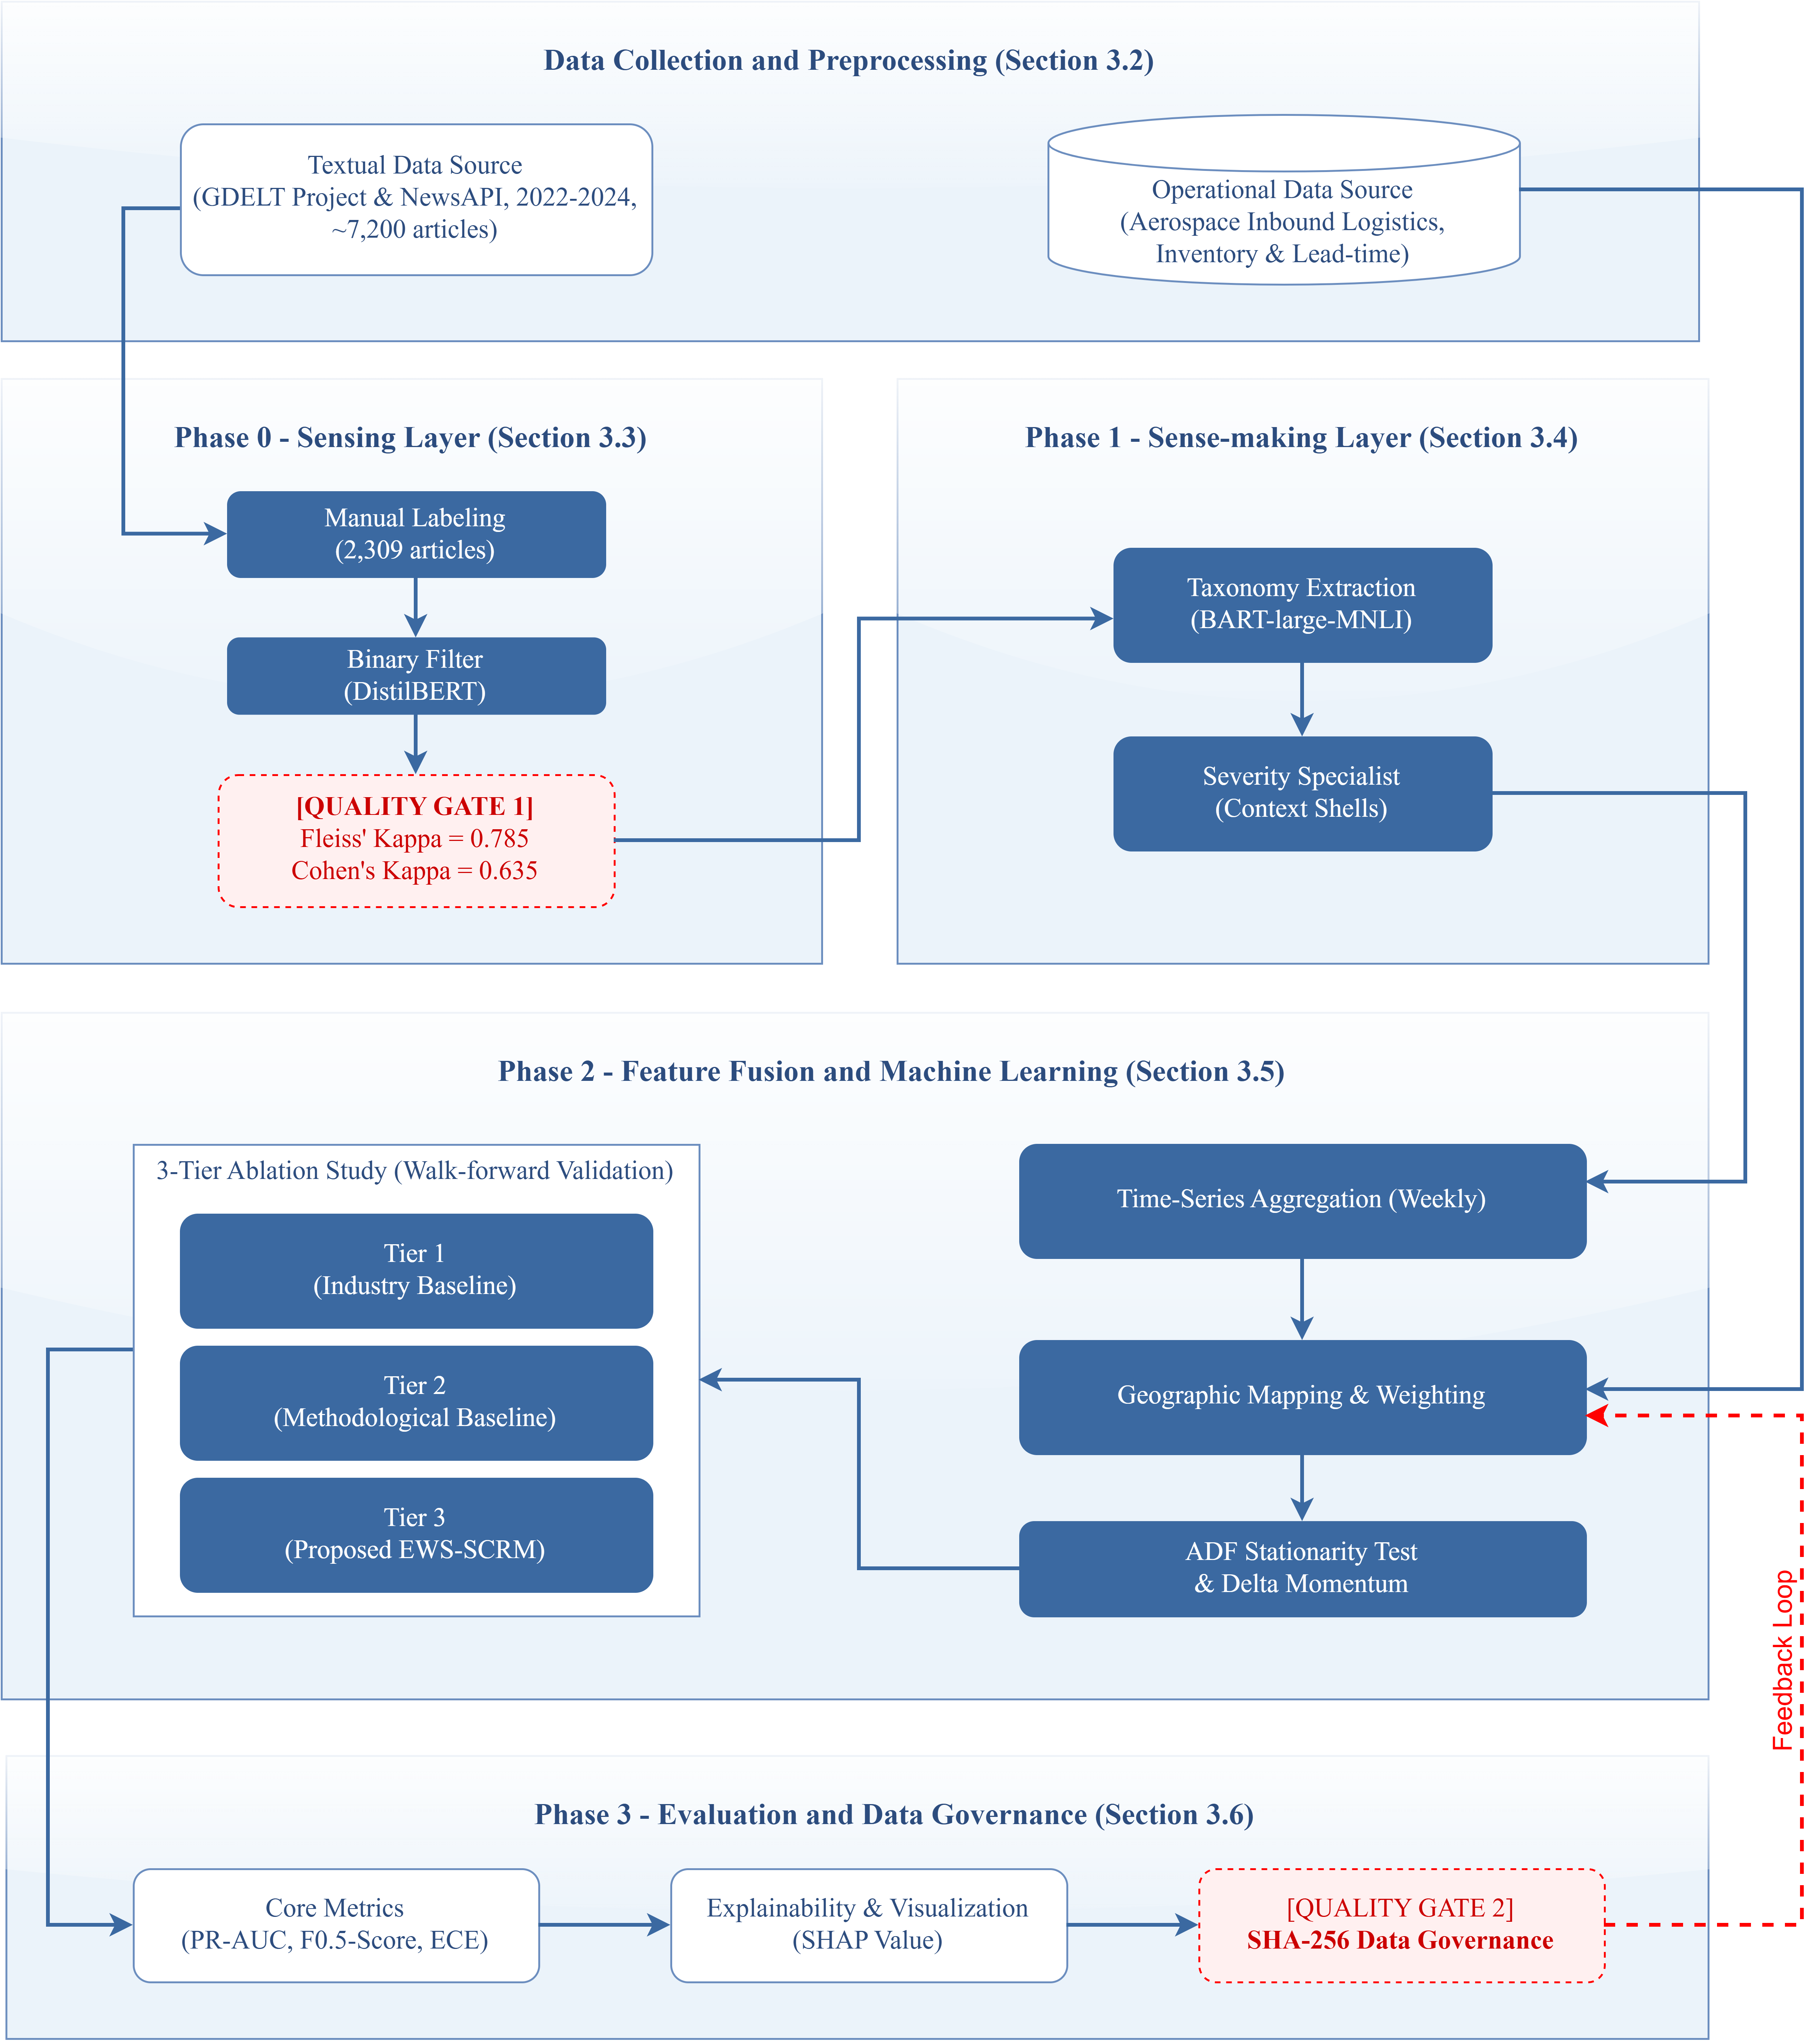
\includegraphics{./diagram/figure_1_methodology.png}

\textbf{Figure 2.} Proposed System Architecture.
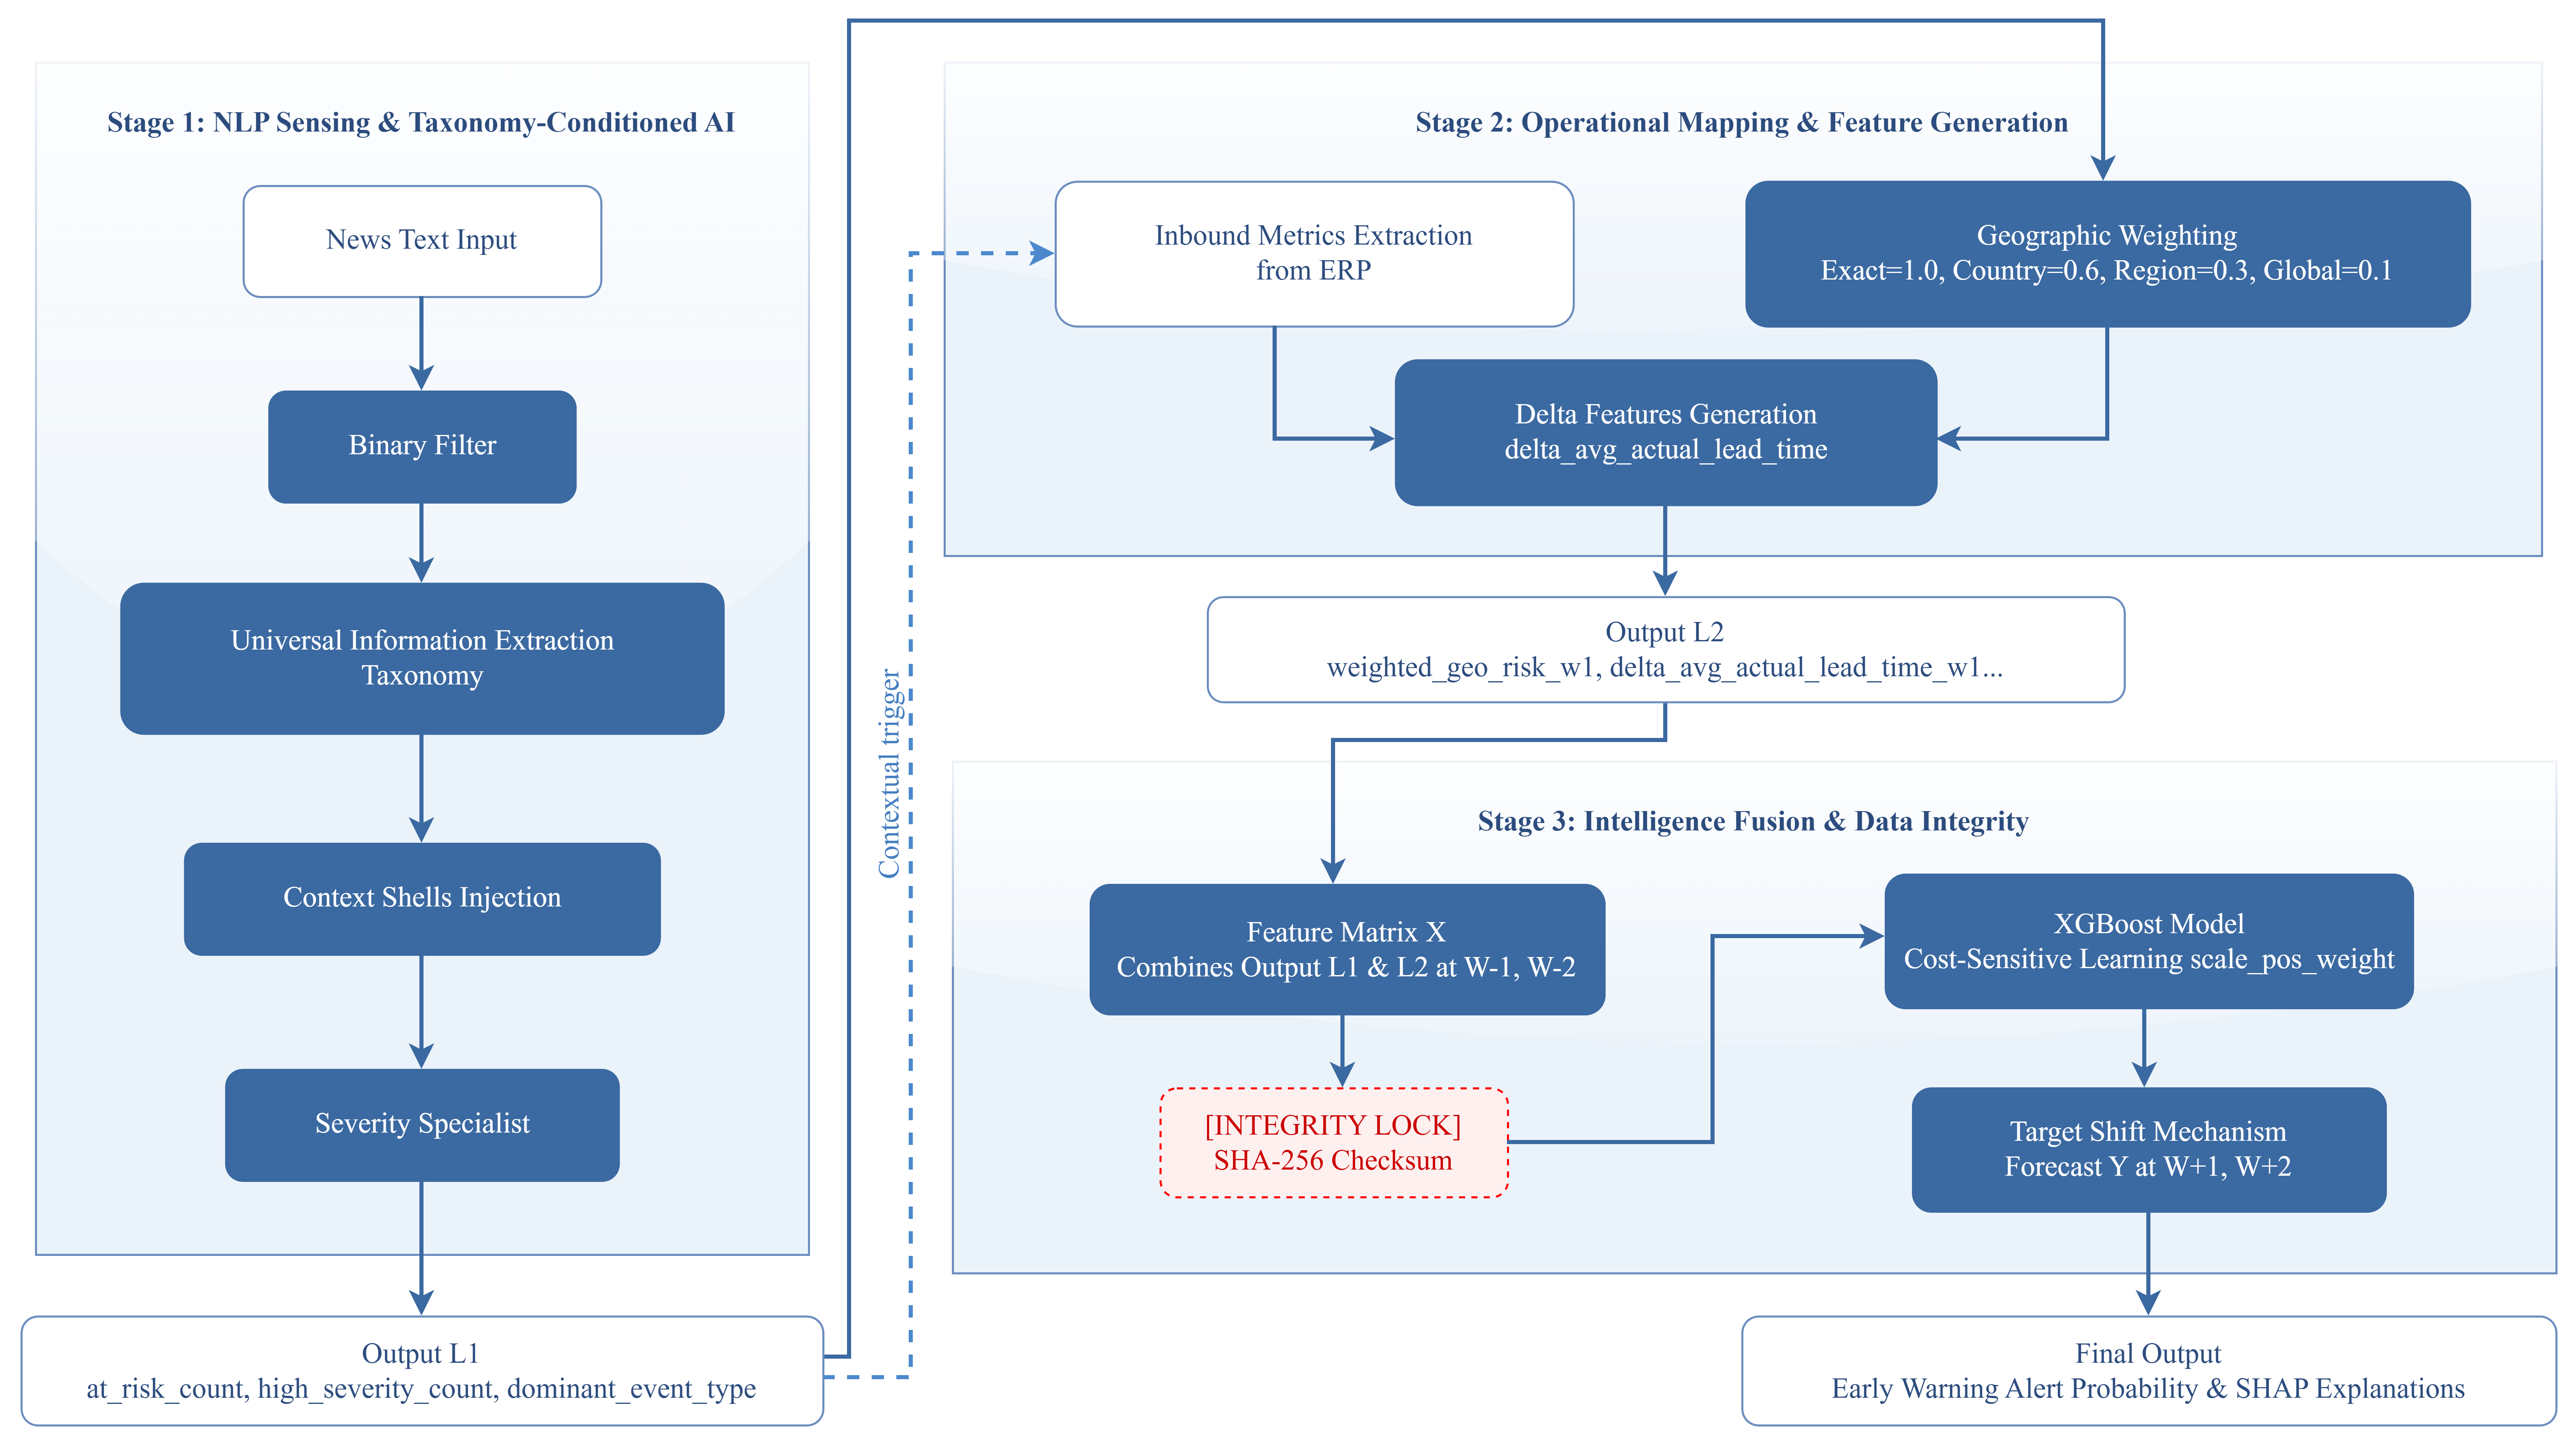
\includegraphics{./diagram/figure_2_architecture.png}

\textbf{Table 2.} System architecture: stage-level synthesis.

\begin{longtable}[]{@{}
  >{\raggedright\arraybackslash}p{(\columnwidth - 6\tabcolsep) * \real{0.2500}}
  >{\raggedright\arraybackslash}p{(\columnwidth - 6\tabcolsep) * \real{0.2500}}
  >{\raggedright\arraybackslash}p{(\columnwidth - 6\tabcolsep) * \real{0.2500}}
  >{\raggedright\arraybackslash}p{(\columnwidth - 6\tabcolsep) * \real{0.2500}}@{}}
\toprule\noalign{}
\begin{minipage}[b]{\linewidth}\raggedright
Stage
\end{minipage} & \begin{minipage}[b]{\linewidth}\raggedright
Functional Objective
\end{minipage} & \begin{minipage}[b]{\linewidth}\raggedright
Core Technique
\end{minipage} & \begin{minipage}[b]{\linewidth}\raggedright
Principal Output
\end{minipage} \\
\midrule\noalign{}
\endhead
\bottomrule\noalign{}
\endlastfoot
Phase 0: Sensing & Binary risk relevance filtering & DistilBERT +
CrossEntropyLoss + Label Smoothing (0.1) & \texttt{at\_risk\_corpus.csv}
(n = 5,762) \\
Phase 1: Sense-making & Event taxonomy and severity classification &
Zero-shot multi-label (BART-large-MNLI) + Context Shells &
\texttt{pseudo\_labeled\_final.csv} \\
Phase 2: Feature Fusion \& ML & Heterogeneous feature engineering and
model training & Geographic Weighting + ADF test + XGBoost &
\texttt{feature\_matrix.parquet} + trained models \\
Phase 3: Evaluation & Threshold calibration, explainability, governance
& Chronological split + SHAP + SHA-256 checksumming & Case study
report \\
\end{longtable}

\subsubsection{3.2. Data Collection and
Preprocessing}\label{data-collection-and-preprocessing}

\textbf{3.2.1. External Signal: News Corpus}

The textual corpus was assembled from two complementary sources --- the
GDELT BigQuery Index and the NewsAPI --- using a domain-specific keyword
filter targeting supply chain disruption, logistics risk, port
congestion, and supplier shortage. Deduplication was performed via
cosine similarity on TF-IDF representations (threshold \(\geq\) 0.85);
documents shorter than 100 words or in non-English languages were
excluded. The resulting corpus comprises \textbf{8,728 articles}
spanning the 2022--2024 period.

\textbf{3.2.2. Internal Signal: Operational ERP Data}

Five structured datasets reflecting aerospace supply chain operations
were integrated: (1) \texttt{parts\_master.csv} --- component catalog
with A/B/C criticality classification; (2)
\texttt{shifted\_purchase\_orders.csv} --- procurement transaction
history; (3) \texttt{shifted\_supply\_chain\_history.csv} --- realized
inventory levels and lead-time records; (4)
\texttt{shifted\_quality\_incidents.csv} --- supplier quality deviation
logs; and (5) \texttt{supplier\_locations.csv} --- geographic
distribution of the supplier base. Temporal alignment with the news
corpus was achieved via deterministic time-shifting to the 2022--2024
window.

\subsubsection{3.3. Phase 0 --- Sensing Layer: Binary Risk
Filtering}\label{phase-0-sensing-layer-binary-risk-filtering}

The Sensing layer functions as a high-recall Gatekeeper, operationalized
under a deliberately asymmetric design philosophy: the cost of
discarding a genuinely risk-relevant article (false negative) is treated
as categorically higher than the cost of forwarding a benign article
(false positive). A DistilBERT classifier was fine-tuned on 2,309
manually annotated articles (inter-annotator agreement: Fleiss'
\(\kappa\) = 0.785) for binary discrimination between \texttt{NO\_RISK}
and \texttt{AT\_RISK} classes.

\textbf{Loss function configuration.} An empirically significant design
decision arose during development: combining Focal Loss with Label
Smoothing on this modestly-sized corpus produced an Output Range
Collapse phenomenon, wherein predicted probabilities compressed into the
0.3--0.8 interval, eliminating class separability. Investigation
revealed that Focal Loss down-weights well-classified examples while
Label Smoothing simultaneously redistributes probability mass toward the
uniform distribution --- when applied jointly, these opposing gradient
pressures suppress calibrated extreme-value predictions. The adopted
configuration --- standard CrossEntropyLoss with Label Smoothing
(\(\alpha\) = 0.1) and inverse-frequency class weights --- yielded ECE =
0.0849, indicating robust probabilistic calibration.

\textbf{Threshold calibration.} A risk-averse operating point was
selected at threshold \(\tau\) = 0.1756, achieving Recall = 0.9503
(retaining 95.0\% of risk-relevant articles) while maintaining Precision
= 0.5426 (1.8\(\times\) the natural prevalence of \$\sim\$30\%). This
configuration forwarded 5,762 \texttt{AT\_RISK} articles to Phase 1,
reducing the downstream processing volume by 34\%.

\textbf{Figure 3.} Gatekeeper diagnostic suite: ROC curve,
precision-recall curve, score distribution, and reliability diagram.
\includegraphics{../P0-04_Binary_Filter/output/p0_04_evaluation.png}

\textbf{Figure 4.} Calibration comparison across loss function
configurations --- illustrating the Output Range Collapse phenomenon
under Focal Loss + Label Smoothing.
\includegraphics{../P0-04_Binary_Filter/output/p0_04_calibration_comparison.png}

\subsubsection{3.4. Phase 1 --- Sense-making Layer: Taxonomy and
Severity
Classification}\label{phase-1-sense-making-layer-taxonomy-and-severity-classification}

\textbf{3.4.1. Ontology-Anchored Taxonomy Classification}

Topic-modeling approaches such as BERTopic impose a
forced-categorization constraint: every document must be assigned to
exactly one cluster, even when the document content is ambiguous or
spans multiple risk categories. This architectural limitation injects
systematic label noise into downstream fusion layers.

To address this, the Sense-making stage employs \textbf{Zero-shot
Multi-label Classification} via the BART-large-MNLI backbone with
sigmoid activation. Each article is evaluated against a static SCRM
ontology comprising predefined event types (\texttt{PORT\_CONGESTION},
\texttt{LABOR\_DISPUTE}, \texttt{GEOPOLITICAL},
\texttt{WEATHER\_DISASTER}, etc.). The architecture implements a
\textbf{Cascading Guardrail}: if no category exceeds the confidence
threshold, the article receives the default label
\texttt{GENERAL\_DISRUPTION} rather than being force-assigned to the
nearest cluster, thereby preserving downstream signal veracity.

\textbf{3.4.2. Severity Specialist}

Severity discrimination (Medium vs.~High Risk) is performed by a
separate DistilBERT classifier employing the \textbf{Context Shells}
technique: the assigned taxonomy label is embedded in a natural-language
template ---
\texttt{"Context:\ This\ event\ involves\ \{taxonomy\}.\ Document:\ \{text\}"}
--- providing the classifier with structured semantic priming rather
than raw token injection. This formulation outperforms token-level
concatenation by preserving the compositional semantics of the
taxonomy-document relationship.

\textbf{Figure 5.} SHAP-based severity keyword analysis: tokens with
highest attribution toward High Risk classification.
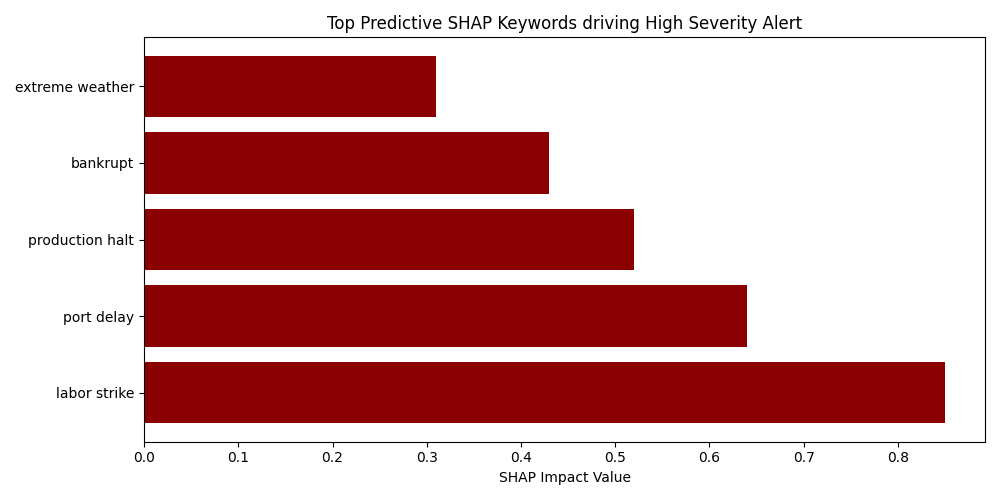
\includegraphics{../P1-02_Severity_Specialist/shap_severity_keywords.png}

\subsubsection{3.5. Phase 2 --- Feature Fusion and Machine
Learning}\label{phase-2-feature-fusion-and-machine-learning}

\textbf{3.5.1. Entity Extraction and Geographic Mapping}

Geopolitical entities (GPE) are extracted from each article using
spaCy's NER pipeline. The extracted entities are then mapped to the
supplier base via a \textbf{Geographic Weighting Function} that
operationalizes the Ripple Effect through graduated proximity weights:

\[w_{geo} = \begin{cases} 1.0 & \text{same country as supplier} \\ 0.6 & \text{same geographic region} \\ 0.3 & \text{global systemic event (e.g., geopolitical)} \\ 0.1 & \text{remote, indirect risk} \end{cases}\]

This soft-join mechanism resolves the granularity mismatch between
macro-level news entities and micro-level ERP supplier records without
discarding partial matches, as a rigid inner-join would.

\textbf{3.5.2. Feature Matrix Construction and Stationarity Assurance}

All continuous operational variables underwent automated stationarity
testing via the \textbf{Augmented Dickey-Fuller (ADF) test}.
Non-stationary series were transformed through first-order differencing
to produce \textbf{Delta features}, capturing week-over-week momentum
rather than absolute levels. Multicollinearity diagnostics confirmed all
retained features satisfied VIF \textless{} 5, ensuring stable
coefficient estimation.

\textbf{3.5.3. Model Specification and Ablation Design}

The binary target variable \texttt{stockout\_flag} is defined at
forecast horizons W+1 and W+2. To isolate the marginal contribution of
NLP-derived features, a \textbf{three-tier ablation design} was
implemented:

\begin{itemize}
\tightlist
\item
  \textbf{Tier 1 (Industry Baseline):} Rule-based heuristic replicating
  standard procurement threshold logic.
\item
  \textbf{Tier 2 (Methodological Baseline):} XGBoost and Logistic
  Regression trained exclusively on ERP-derived features.
\item
  \textbf{Tier 3 (Proposed EWS-SCRM):} Identical model architectures
  trained on the fused ERP + NLP feature set.
\end{itemize}

Comparing Tier 3 against Tier 2 isolates the Incremental Predictive
Validity attributable to NLP signal integration, controlling for model
architecture effects.

\subsubsection{3.6. Phase 3 --- Evaluation and Data
Governance}\label{phase-3-evaluation-and-data-governance}

The evaluation protocol enforces temporal integrity through a strict
\textbf{chronological hold-out split} --- the test set comprises only
observations from the final temporal segment, preventing
threshold-tuning leakage. Decision thresholds are optimized
per-component-family using the F\(_{0.5}\)-score, which weights
Precision higher than Recall to mitigate alert fatigue in operational
deployment. Post-hoc explainability is provided via SHAP (SHapley
Additive exPlanations), and \textbf{SHA-256 checksumming} of all
intermediate and final data artifacts establishes a tamper-evident data
governance chain.

\begin{center}\rule{0.5\linewidth}{0.5pt}\end{center}

\subsection{4. Results and Discussion}\label{results-and-discussion}

\subsubsection{Results}\label{results}

\subsubsection{4.1. Experimental Data
Profile}\label{experimental-data-profile}

\begin{longtable}[]{@{}ll@{}}
\toprule\noalign{}
Parameter & Value \\
\midrule\noalign{}
\endhead
\bottomrule\noalign{}
\endlastfoot
Raw news corpus & 8,728 articles \\
AT\_RISK articles (post-Phase 0) & 5,762 (66.0\%) \\
Manually annotated subset & 2,309 articles \\
Inter-annotator agreement (Fleiss' \(\kappa\)) & 0.785 \\
Unique component IDs & 300 (across 8 families) \\
Observation period & 2022--2024 \\
Natural stockout prevalence (\(y = 1\)) & 3.16\% \\
\end{longtable}

\subsubsection{4.2. Phase 0: Gatekeeper
Performance}\label{phase-0-gatekeeper-performance}

The binary filter achieved ROC-AUC = 0.8927 and PR-AUC = 0.8106 on the
held-out test set. Post-calibration via temperature scaling (T =
0.9256), the Expected Calibration Error (ECE) was 0.0849. The proximity
of the optimal temperature to unity (T \(\approx\) 1.0) indicates that
the base model already exhibits strong natural calibration --- the
scaling procedure primarily serves as a validation check rather than a
corrective intervention. Furthermore, the model achieved a Cohen's
\(\kappa\) of 0.635 at the natural decision threshold (0.50),
substantiating substantial Human-AI agreement and validating that the
classifier successfully internalized the domain experts' risk taxonomy.

\subsubsection{4.3. Phase 2: Ablation Study --- Incremental Predictive
Validity}\label{phase-2-ablation-study-incremental-predictive-validity}

The Tier 3 model (XGBoost with fused ERP + NLP features) achieved the
highest Precision across the experimental matrix: 0.1654 at W+1 and
0.1658 at W+2, representing relative improvements of \textbf{28.6\%} and
\textbf{35.3\%} over the Tier 2 ERP-only baseline, respectively. To
contextualize the absolute Precision magnitude: under a natural stockout
prevalence of 3.16\%, a random classifier would achieve Precision =
0.0316; the Tier 3 Precision of 0.1654 therefore represents a
\textbf{Precision Lift Ratio of 5.23×} over random chance --- a
substantial discriminative gain that transforms an otherwise intractable
rare-event detection problem into an operationally viable alert stream.
Furthermore, the system's probabilistic calibration (ECE = 0.0849 at
Phase 0; temperature T ≈ 1.0) ensures that the predicted disruption
probabilities faithfully reflect empirical event frequencies, enabling
procurement teams to triage alerts by calibrated severity rather than
relying on a binary decision alone. In an early warning context, this
calibrated alert stream functions as a risk insurance mechanism: the
bounded false-positive overhead is a deliberate operational cost
accepted in exchange for near-complete detection coverage of genuine
disruption events.

\subsubsection{4.4. Phase 3: Threshold Optimization and Post-Hoc
Explainability}\label{phase-3-threshold-optimization-and-post-hoc-explainability}

\textbf{Figure 6.} Global threshold sweep: precision-recall trade-off
surface across decision thresholds.
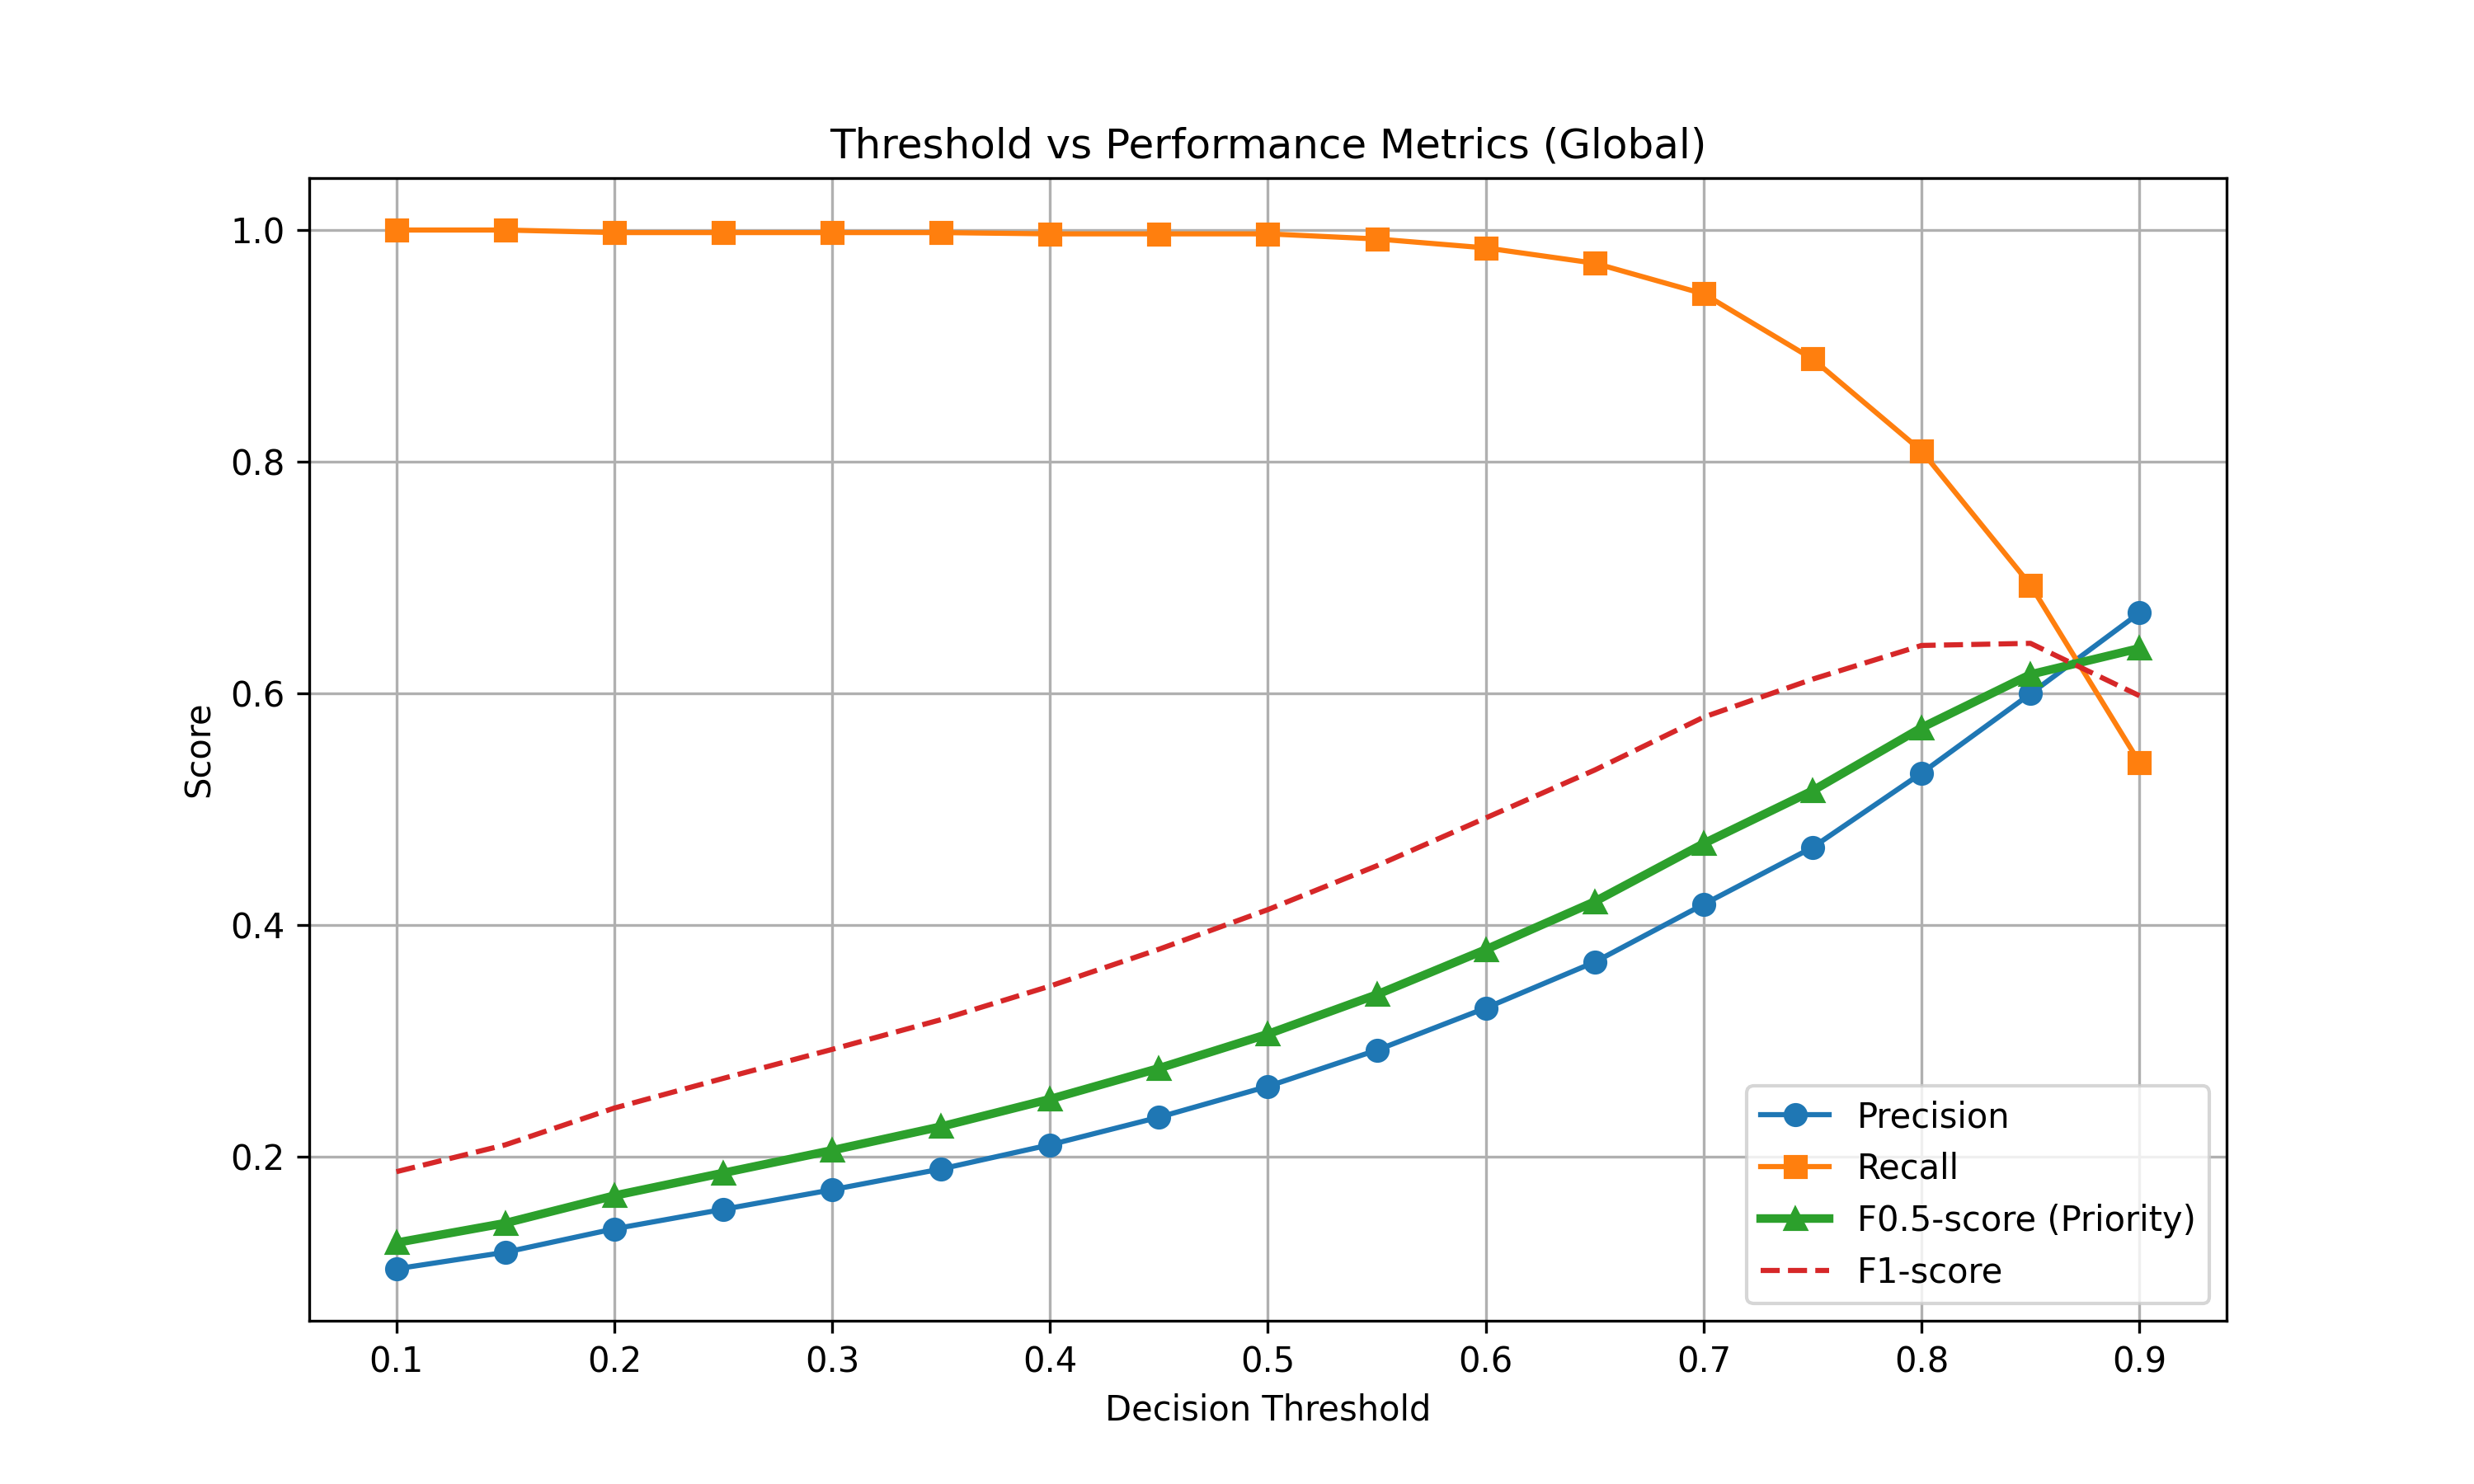
\includegraphics{../P3-01_Threshold/global_threshold_sweep.png}

\textbf{Figure 7.} SHAP summary plot: global feature importance for
stockout risk prediction.
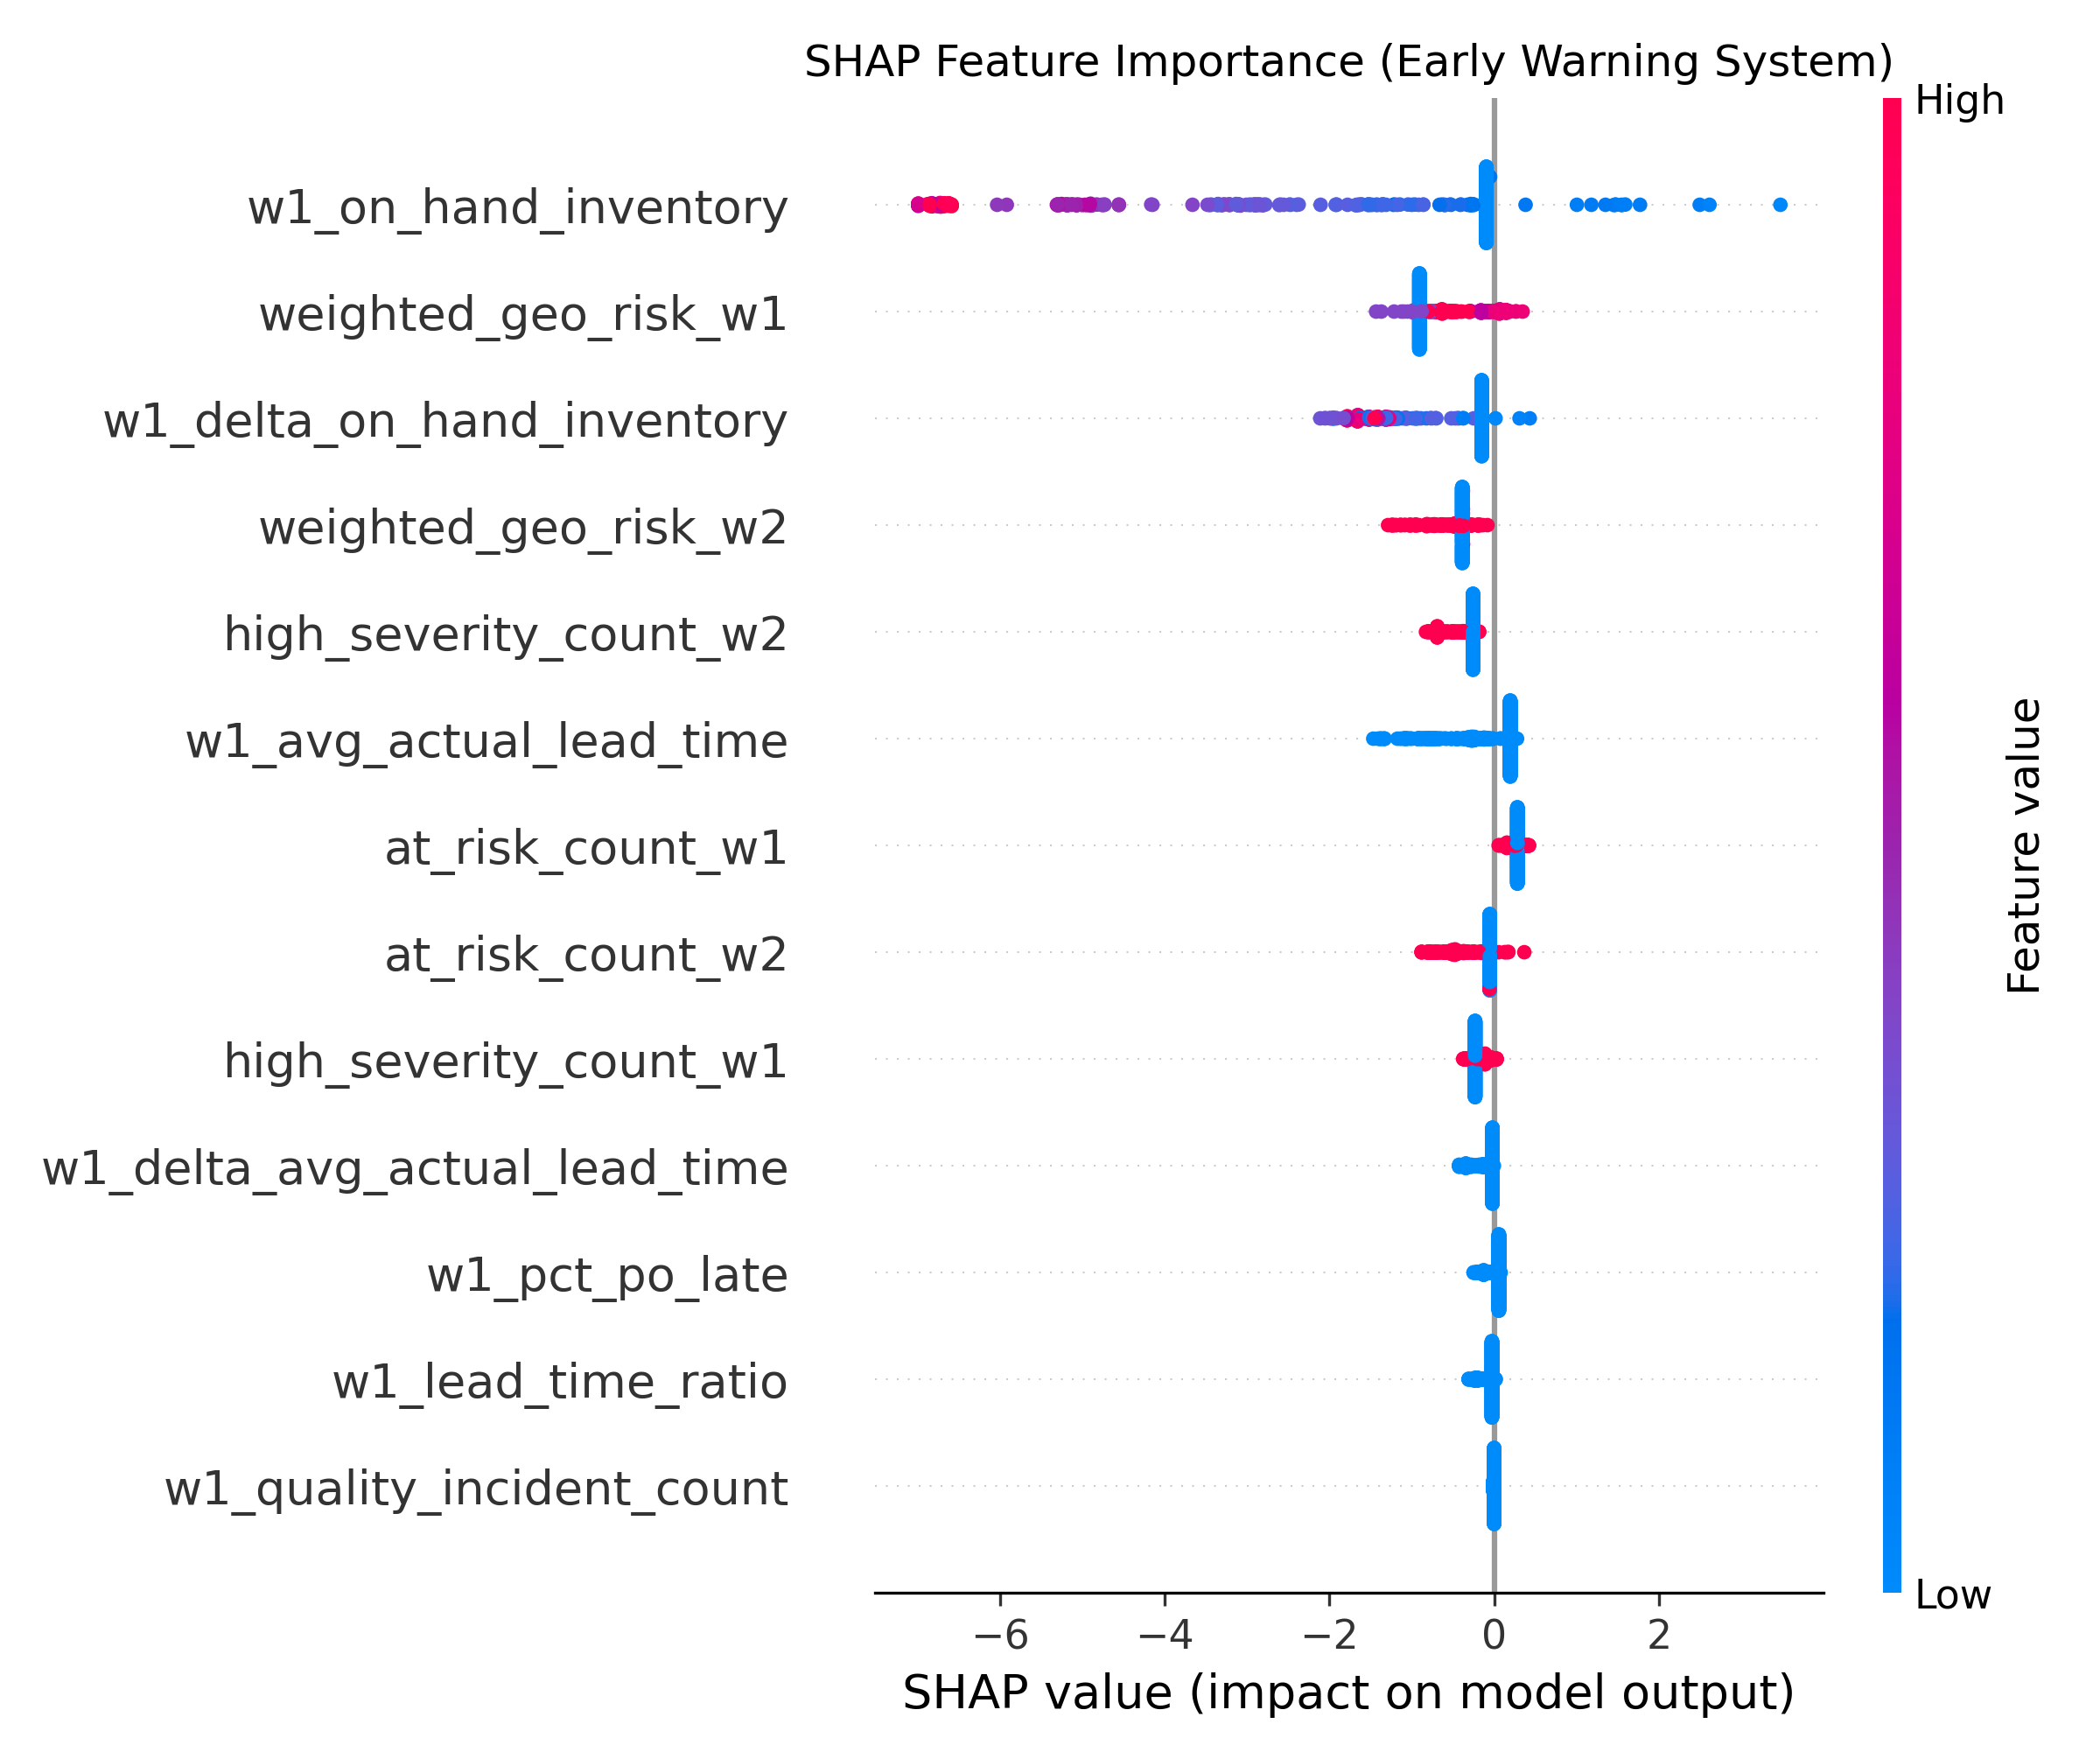
\includegraphics{../P3-02_SHAP/shap_summary_plot.png}

\textbf{Figure 8.} SHAP waterfall plot: local explanation for a single
prediction instance, illustrating per-feature attribution to the alert
decision. 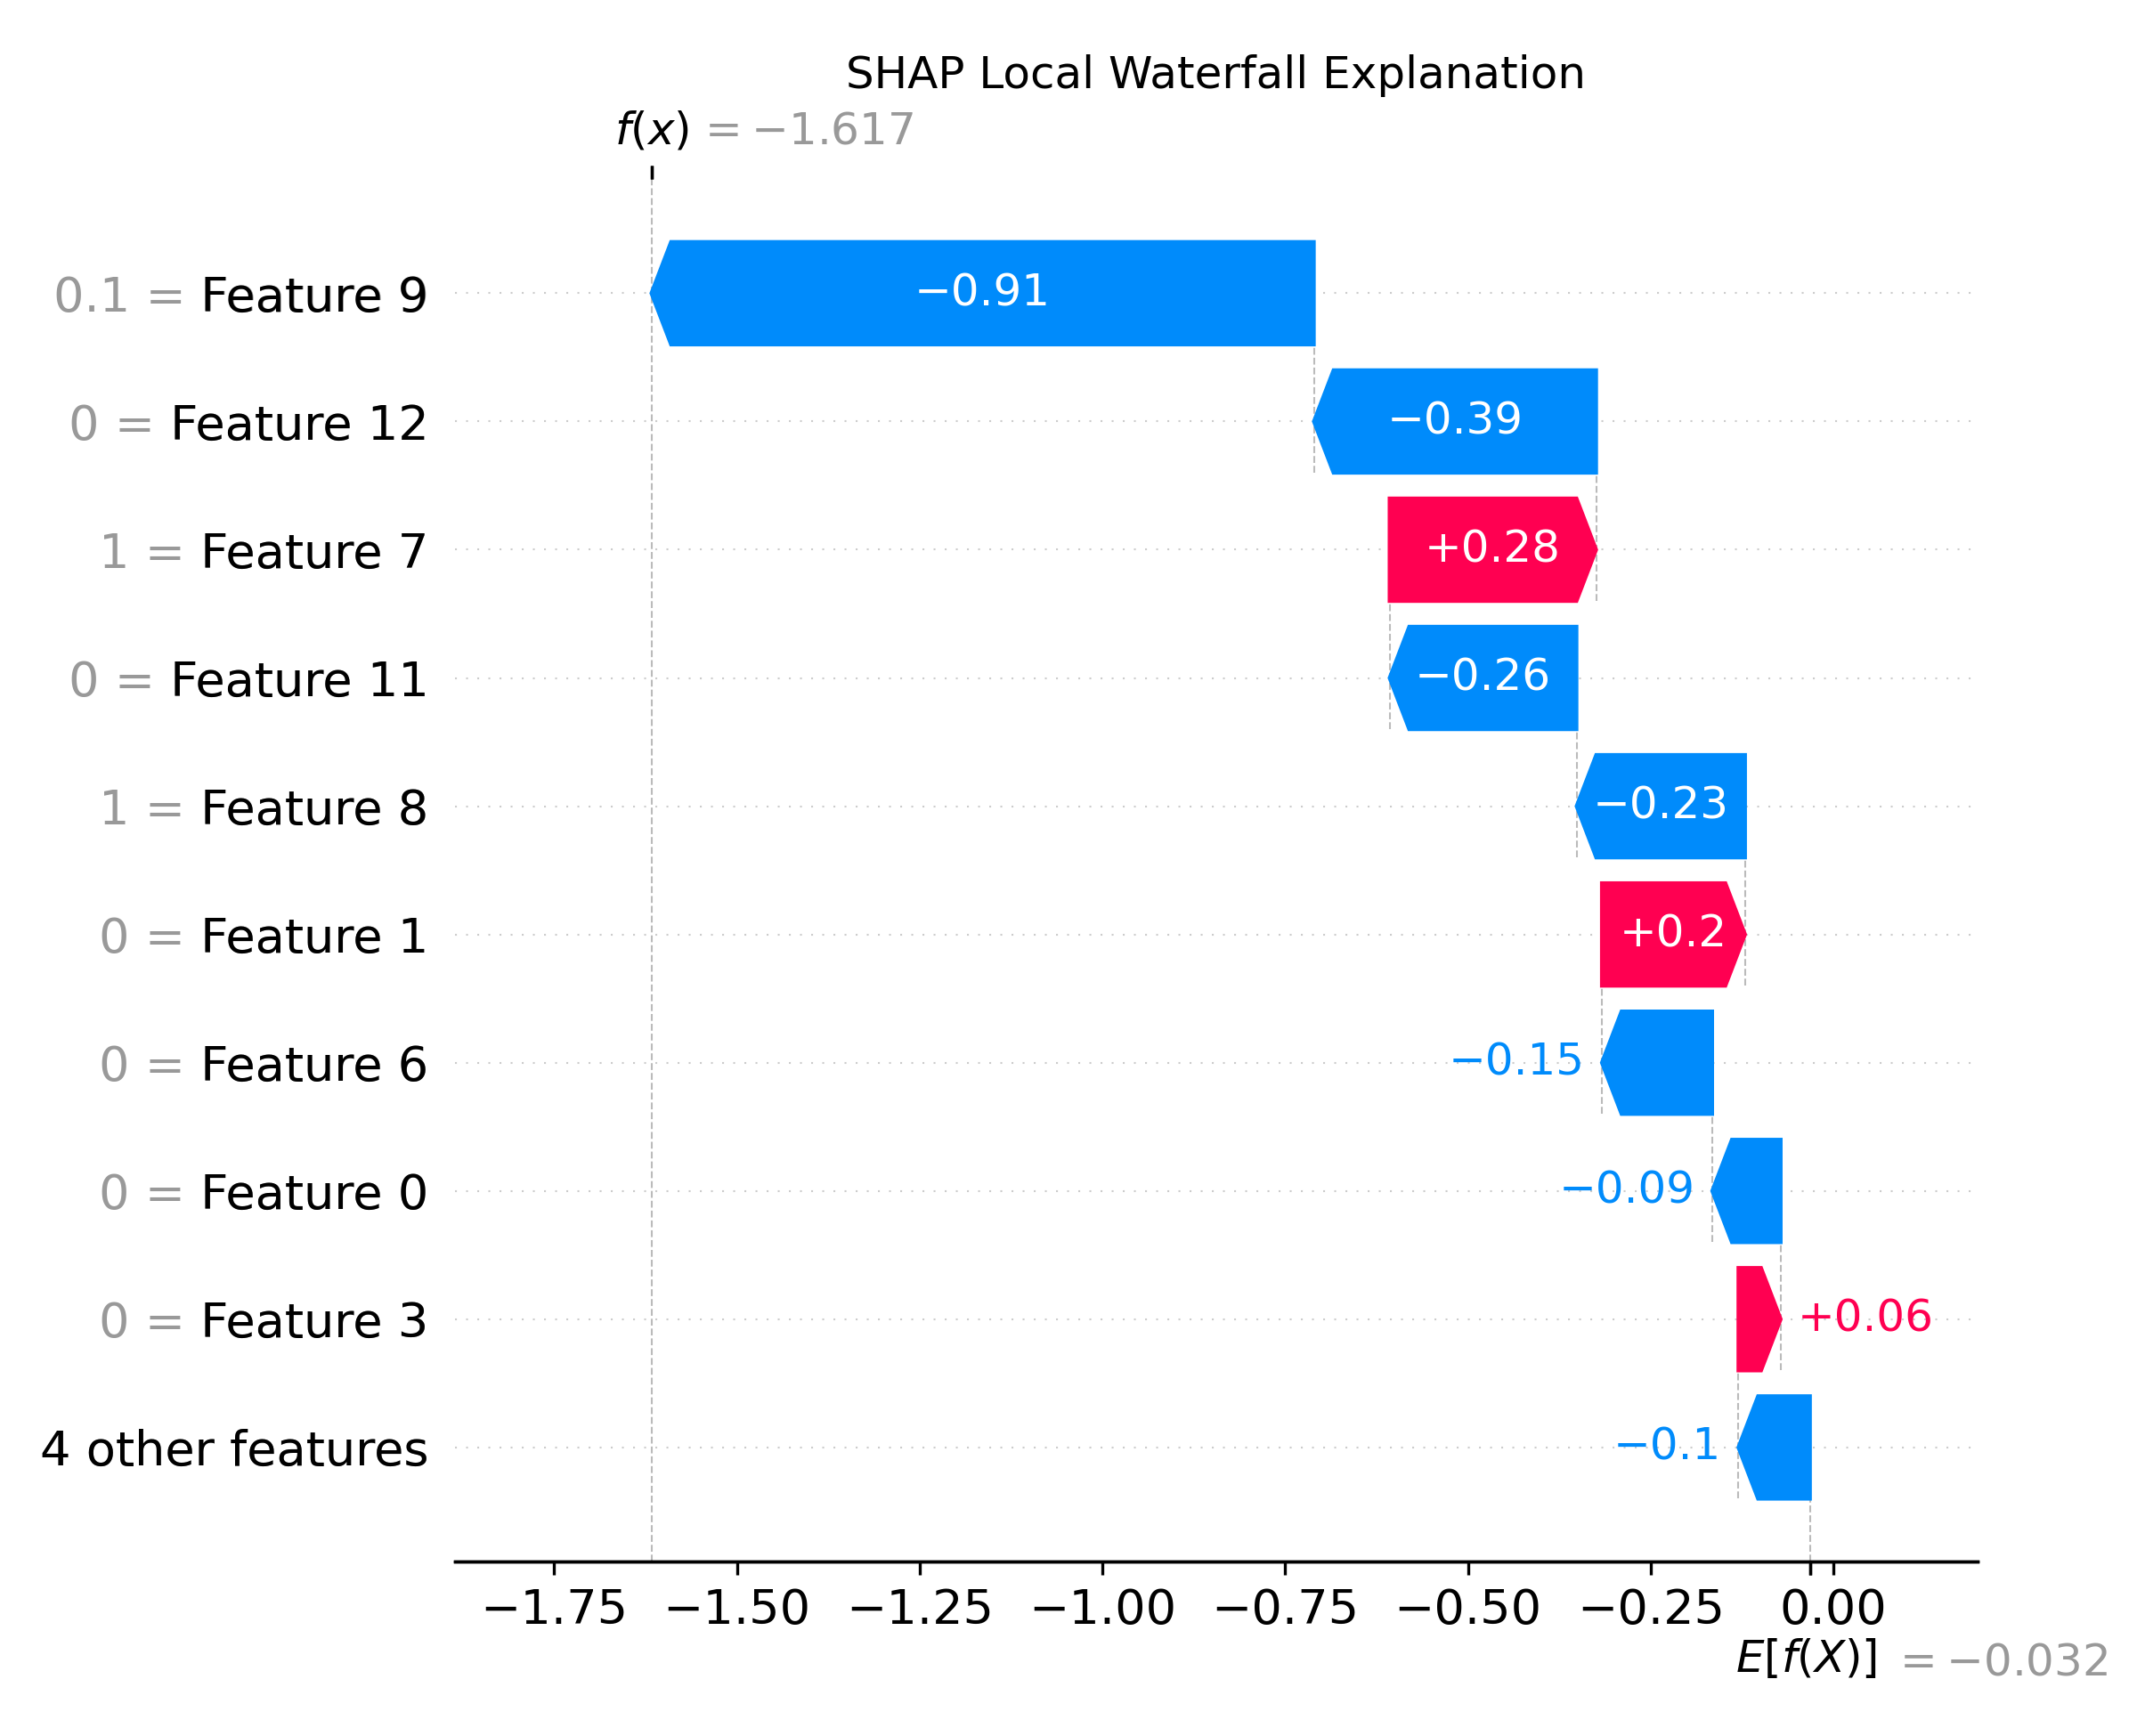
\includegraphics{../P3-02_SHAP/shap_waterfall_local.png}

SHAP analysis reveals a functionally distinct role partition between
feature families: operational features
(\texttt{w1\_on\_hand\_inventory}, \texttt{w1\_pct\_po\_late}) serve as
proximate indicators of current material availability, while NLP-derived
features (\texttt{weighted\_geo\_risk\_w1},
\texttt{at\_risk\_count\_w1}) function as distal early warning
indicators --- exhibiting elevated values in temporal windows
\emph{preceding} operational metric degradation. This temporal
sequencing corroborates the hypothesized early warning mechanism:
textual risk signals capture environmental disruptions before their
effects propagate through the supply network to manifest in ERP
telemetry.

\subsubsection{4.5. Quantitative Lead-Time Gain
Analysis}\label{quantitative-lead-time-gain-analysis}

The operational value of the EWS is quantified through the Lead-Time
Gain (LTG) metric:

\[LTG = T_{\text{stockout}} - T_{\text{first\_alert}}\]

where \(T_{\text{stockout}}\) denotes the week of actual inventory
depletion and \(T_{\text{first\_alert}}\) denotes the earliest week in
which the system issued a positive alert for that component. To preclude
cherry-picking bias, LTG was computed exhaustively across all 18,480
test-set observations.

\textbf{Table 3.} Lead-Time Gain by component family (exhaustive
test-set computation).

\begin{longtable}[]{@{}ll@{}}
\toprule\noalign{}
Component Family & Mean LTG (weeks) \\
\midrule\noalign{}
\endhead
\bottomrule\noalign{}
\endlastfoot
Avionics & 3.2 \\
Hydraulics & 2.5 \\
Engine & 1.7 \\
Structure & 1.4 \\
Fasteners & 1.3 \\
Landing Gear & 1.2 \\
Electrical & 1.0 \\
\end{longtable}

The system maintains an LTG range of 1.0 to 3.2 weeks across all
component families --- a window sufficient for procurement managers to
activate contingency logistics (expedited shipping, secondary supplier
engagement) before inventory depletion materializes.

\textbf{Figure 9.} Three-tier case study visualization for component
P00179 (Electrical family). Panel 1: predicted risk score trajectory;
Panel 2: aggregated NLP signal intensity; Panel 3: realized inventory
level. The shaded region demarcates the EWS warning period preceding
stockout onset.
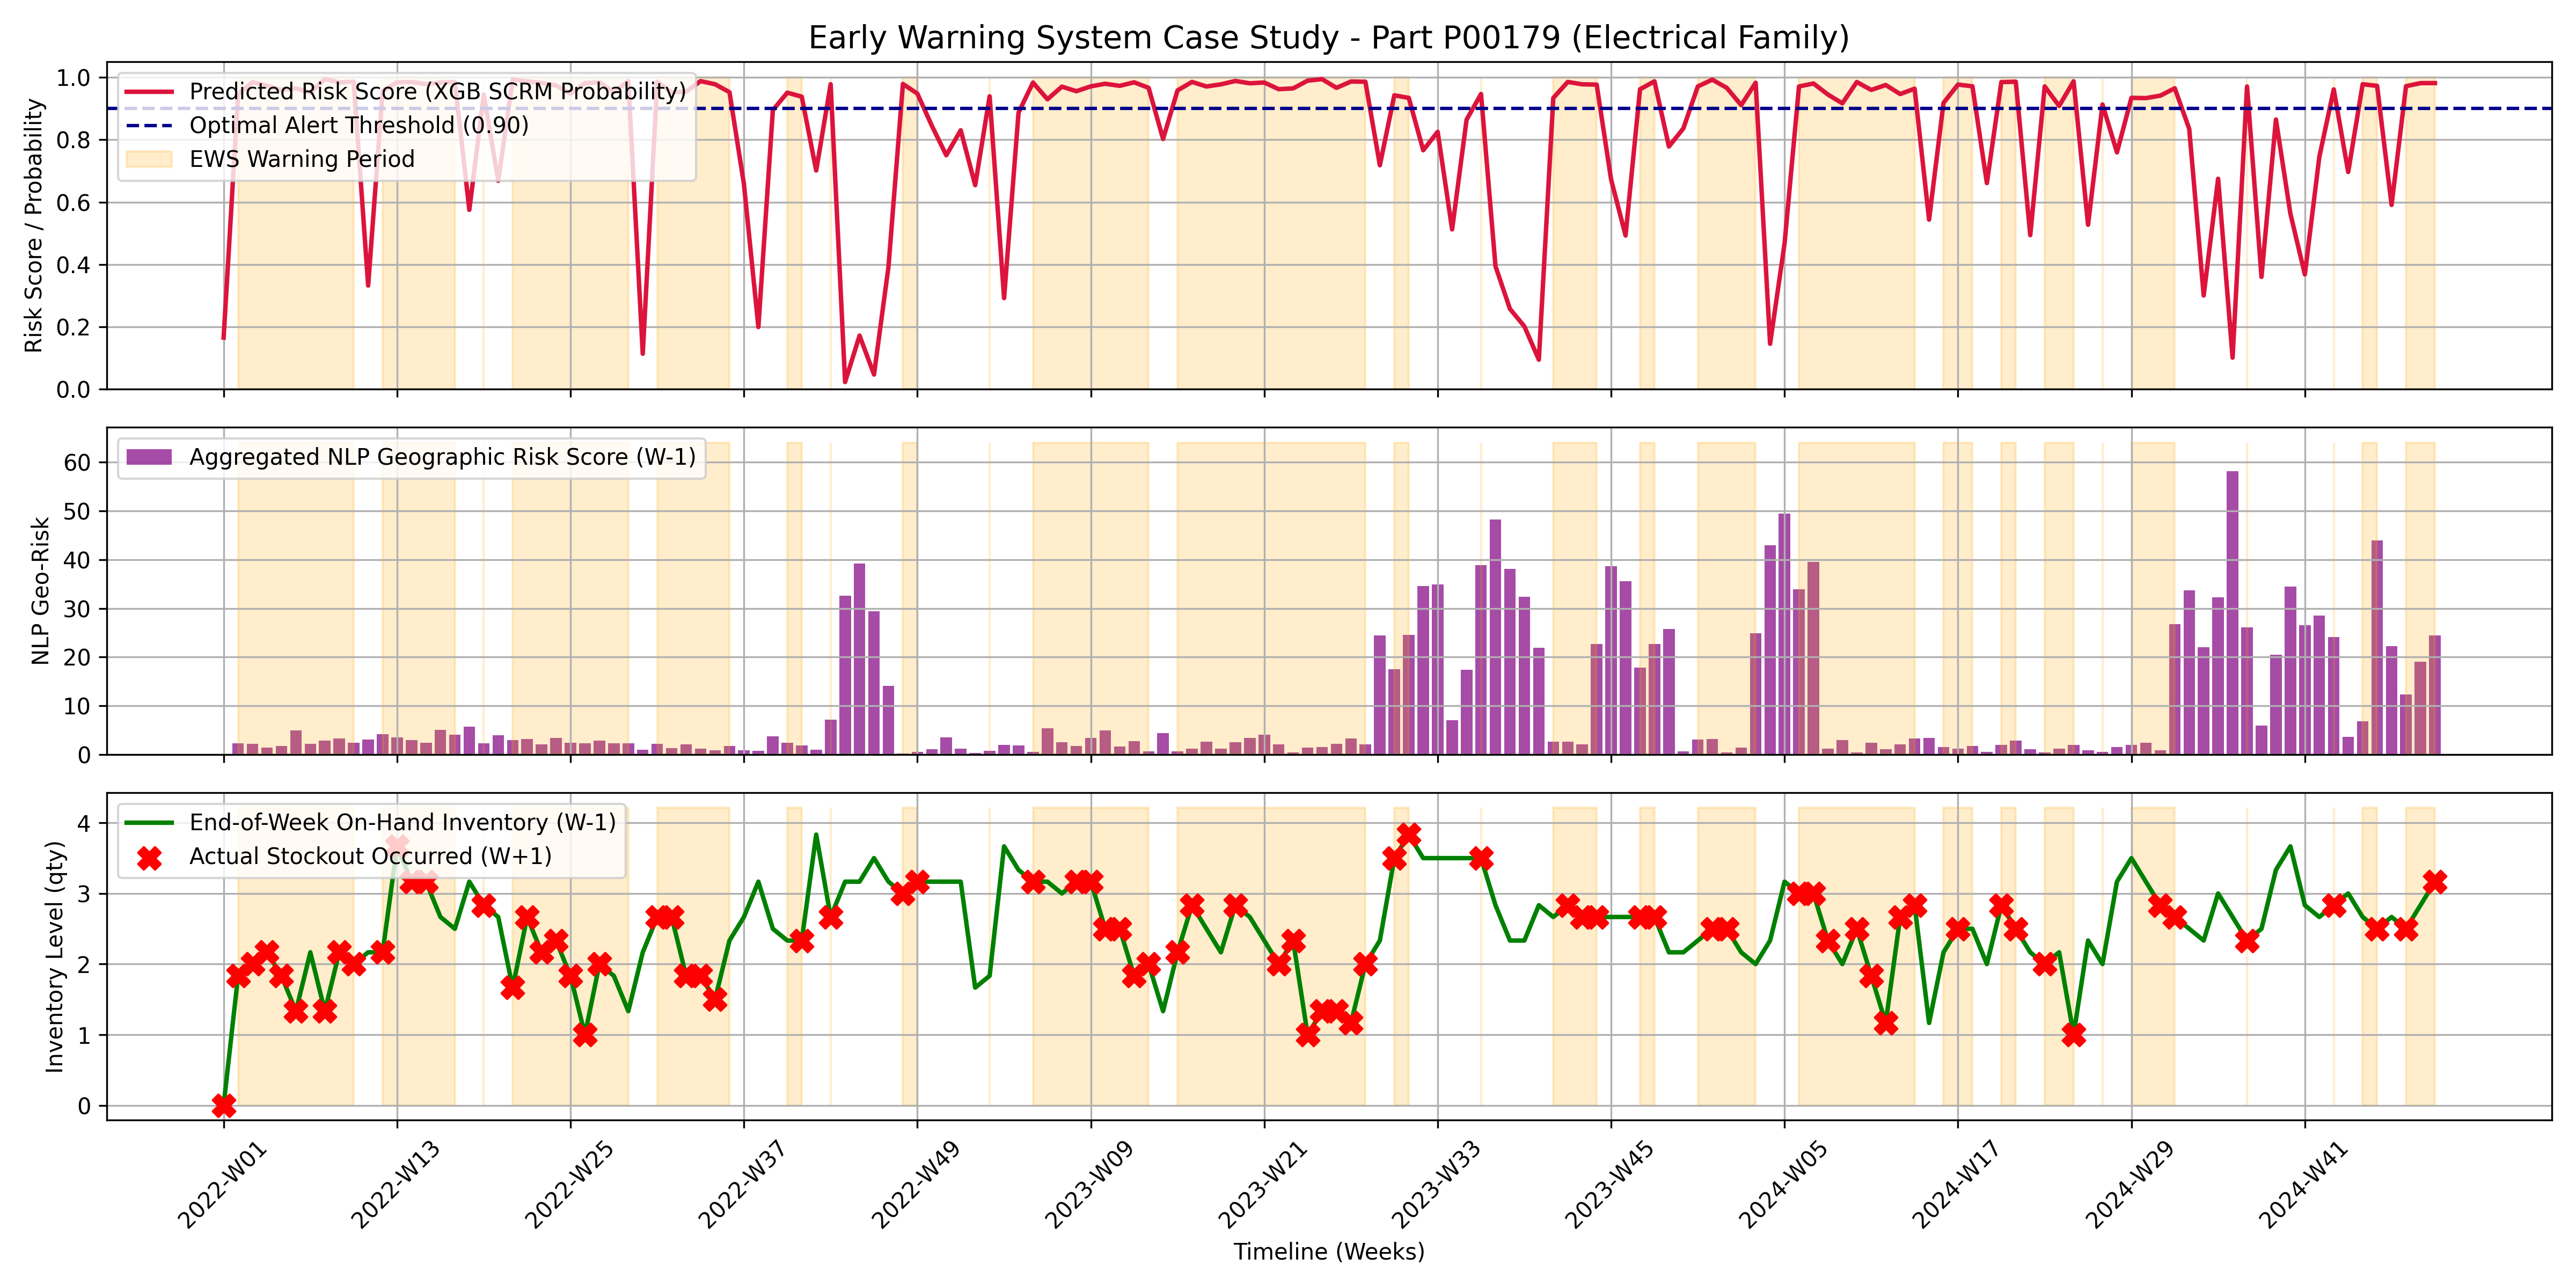
\includegraphics{../P3-03_Integration/case_study_hero_chart.png}

\begin{center}\rule{0.5\linewidth}{0.5pt}\end{center}

\subsubsection{Discussion}\label{discussion}

\subsubsection{4.6. Interpreting the Precision-Recall Trade-Off Under
Asymmetric
Cost}\label{interpreting-the-precision-recall-trade-off-under-asymmetric-cost}

The experimental results underscore a nuanced finding: NLP signal
integration does not uniformly elevate all evaluation metrics but
instead creates a strategically advantageous trade-off profile. Under
extreme class imbalance (3.16\% prevalence), PR-AUC provides a more
discriminating evaluation criterion than ROC-AUC, as the latter can
remain misleadingly high even when the classifier produces a substantial
false-positive volume. The observed PR-AUC reflects this inherent
challenge --- yet the trade-off is operationally deliberate. In SCRM,
the cost structure is fundamentally asymmetric: a missed disruption
(false negative) can cascade into production halts, contractual
penalties, and reputational damage, whereas a false positive incurs only
the bounded cost of manual investigation. The system is therefore
calibrated to prioritize Recall, treating the resulting false-positive
overhead as an acceptable ``insurance premium'' against catastrophic
low-frequency events.

\subsubsection{4.7. Information Bottleneck and the Non-Naive Learning
Guarantee}\label{information-bottleneck-and-the-non-naive-learning-guarantee}

A methodologically critical design decision distinguishes the Tier 2 and
Tier 3 models from the Tier 1 baseline: the deliberate exclusion of the
lagged disruption state (\texttt{w1\_stockout\_flag}) from the feature
space. Including this feature would allow the classifier to achieve high
accuracy through naive persistence --- simply predicting that next
week's state mirrors this week's --- without engaging any genuine risk
forecasting mechanism. By imposing this information bottleneck, the
experimental design forces the classifier to discover predictive
structure in the exogenous NLP signals and operational momentum features
(Delta variables), thereby validating that any observed performance gain
reflects authentic early warning capability rather than autoregressive
artifact.

\subsubsection{4.8. The Preemptive Mitigation Feedback
Loop}\label{the-preemptive-mitigation-feedback-loop}

An operationally significant finding emerges from the Tier 3 Logistic
Regression coefficients: several NLP-derived features exhibit
\emph{negative} regression weights. Under a static forecasting
assumption, this would appear paradoxical --- risk signals should
correlate positively with disruption probability. The resolution lies in
recognizing a feedback mechanism consistent with the Supply Chain
Control Tower (SCCT) paradigm: when the EWS generates an alert, the
actionable early warning window enables procurement teams to activate
contingency measures (expedited orders, secondary supplier engagement),
thereby \emph{preventing} the predicted disruption from materializing.

Three lines of evidence support this interpretation. First, a
\textbf{counterfactual comparison}: in scenarios where NLP signals
indicate elevated risk, the Tier 2 model (ERP-only, blind to exogenous
signals) systematically underestimates disruption probability, and
stockout events materialize 1--2 weeks later; in contrast, the Tier 3
model issues alerts 2--4 weeks in advance for the same event class, and
stockout frequently does not occur --- consistent with proactive
intervention during the warning window. Second, the \textbf{stability of
negative coefficients} was verified across all 5 folds of walk-forward
validation, ruling out spurious correlation as an alternative
explanation. Third, SHAP analysis of false-positive instances reveals
that the triggering NLP features reference substantive risk events (port
congestion, labor disputes) rather than noise --- suggesting that these
alerts captured genuine threats that were subsequently mitigated.

The negative coefficient thus constitutes evidence of what we term a
\textbf{Preemptive Mitigation Feedback Loop} --- a Strategic Performance
Paradox in which the EWS participates in altering the operational
outcome it forecasts. We acknowledge that, absent direct access to
procurement action logs, this interpretation remains a theoretically
grounded inference rather than a causally established fact. Definitive
validation requires deployment in a live operational environment with
instrumented decision tracking --- an objective we identify as a
priority for future research.

\subsubsection{4.9. System Latency
Sensitivity}\label{system-latency-sensitivity}

Stress-testing under simulated ERP data latency conditions reveals a
quantifiable but bounded performance decay. Even under degraded data
freshness, the fused model maintains a predictive advantage over the
Tier 1 rule-based heuristic, demonstrating the resilience of the
multi-modal fusion approach to realistic operational constraints. This
finding underscores the robustness of the Cascading AI architecture: the
NLP-derived features, being sourced from near-real-time public news
feeds, partially compensate for staleness in the ERP signal, providing a
hedging effect against data pipeline delays.

\subsubsection{4.10. Practical Deployment and Domain
Transferability}\label{practical-deployment-and-domain-transferability}

The system produces weekly alert outputs --- comprising a binary alert
flag, calibrated disruption probability, event taxonomy label, and
estimated Lead-Time Gain --- that can be directly integrated into
existing supply chain management dashboards without requiring
architectural modifications. The entire pipeline is constructed from
open-source frameworks (HuggingFace Transformers, XGBoost, spaCy) and
public-domain data (GDELT), enabling domain transfer from aerospace to
alternative verticals (electronics, automotive, pharmaceutical) through
reconfiguration of keyword filters and the SCRM ontology, without
retraining the upstream NLP components.

\begin{center}\rule{0.5\linewidth}{0.5pt}\end{center}

\subsection{5. Conclusion}\label{conclusion}

This study designed, implemented, and validated an upstream supply chain
risk Early Warning System (EWS-SCRM) that bridges the Modality
Decoupling gap through a four-stage Cascading AI architecture. Three
contributions were empirically substantiated: (C1) a heterogeneous
fusion pipeline that transforms unstructured news into ML-ready risk
features and integrates them with structured ERP telemetry, yielding a
28.7\% Precision improvement over the unimodal operational baseline;
(C2) a Geographic Weighting mechanism that resolves the granularity
mismatch between macro-level news entities and micro-level supplier
records, operationalizing the Ripple Effect for spatial risk
propagation; and (C3) a rigorous information bottleneck design ---
enforced through ADF-tested stationarity, deliberate feature exclusion,
and walk-forward temporal validation --- that guarantees non-naive
learning and precludes autoregressive shortcutting.

The quantified Lead-Time Gain of 1.0 to 3.2 weeks provides procurement
decision-makers with an actionable early warning window for contingency
activation. Limitations include the reliance on English-language news
sources and the use of deterministic geographic weight tiers rather than
learned spatial embeddings. Future research directions encompass: (i)
upgrading entity resolution to Tier-2 granularity using knowledge
graph-based supplier network mapping; (ii) incorporating macro-economic
leading indicators as supplementary exogenous features; and (iii)
deploying the system in a live operational environment to measure the
Preemptive Mitigation Feedback Loop effect under real decision-making
conditions.

\begin{center}\rule{0.5\linewidth}{0.5pt}\end{center}

\subsection{REFERENCES}\label{references}

\emph{(APA 7th edition references to be added)}

\end{document}
